\section{Timestamps}

Locking is also named pessimistic concurrency control because it assumes that collisions will arise but in reality collisions are rare. 

So, it is possible to use optimistic concurrency control methods like timestamps, which are identifier that defines a total ordering of the events of a system. Each transaction has a timestamp representing the time 
at which the transaction begins so that transactions can be ordered: the smaller is the index the older is the transaction. A schedule is accepted only if it reflects the serial 
ordering of the transactions induced by their timestamps. The timestamps are given by a system's function on request. The syntax of a timestamp is the following: 
\[\textnormal{event-id}.\textnormal{node-id}\]
The algorithm's synchronization is based on send-receive of messages, and it is called Lamport method: it is not possible to receive a message 
from the future, if this happens the bumping rule is used to bump the timestamp of the receive event beyond the timestamp of the send event.     
\begin{example}
    An example of timestamps assignation at two different nodes can be the following. 
    \begin{figure}[H]
        \centering
        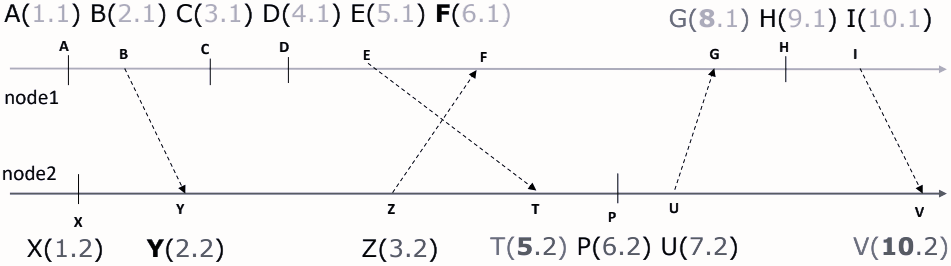
\includegraphics[width=0.75\linewidth]{images/timestamps.png}
    \end{figure}
\end{example}
The scheduler uses two counters: one for writes WTM($x$) and another for reads RTM($x$). The scheduler receives read/write requests tagged with the timestamp of the 
requesting transaction. In case of a read operation we can have: 
\begin{itemize}
    \item If $ts<\textnormal{WTM}(x)$ the request is rejected and the transaction is killed. 
    \item Else, access is granted, and we set $\textnormal{RTM}(x)=\max(\textnormal{RTM}(x),ts)$. 
\end{itemize}
In case of a write operation we can have: 
\begin{itemize}
    \item If $ts<\textnormal{RTM}(x)$ or $ts<\textnormal{WTM}(x)$ the request is rejected, and the  transaction is killed. 
    \item Else, access is granted, and we set $\textnormal{WTM}(x)=ts$. 
\end{itemize}
The previous rules cause too many transaction killings. 
\begin{example}
    Let us assume $\textnormal{RTM}(x)=7$ and $\textnormal{WTM}(x)=4$ and the following schedule: 
    \[S=r_6(x) r_8(x) r_9(x) w_8(x) w_{11}(x) r_{10}(x)\]
    Using the timestamps we obtain: 
    \begin{table}[H]
        \centering
        \begin{tabular}{ccc}
        \textbf{Request} & \textbf{Response} & \textbf{New value} \\ \hline
        $r_6(x)$         & $\checkmark$      & -                  \\
        $r_8(x)$         & $\checkmark$      & $\textnormal{RTM}(x)=8$         \\
        $r_9(x)$         & $\checkmark$      & $\textnormal{RTM}(x)=9$         \\
        $w_8(x)$         & $\tikzxmark$      & $T_8$ killed       \\
        $w_{11}(x)$      & $\checkmark$      & $\textnormal{WTM}(x)=11$        \\
        $r_{10}(x)$      & $\tikzxmark$      & $T_{10}$ killed   
        \end{tabular}
    \end{table}
\end{example}
It is not possible to compare 2PL to TS (this means that there is no subset between the categories). We have only that TS implies CSR. 
\begin{proof}[TS implies CSR]
    Let $S$ be a TS schedule of $T_1$ and $T_2$. Suppose $S$ is not CSR, which implies that it contains a cycle between $T_1$ and $T_2$. $S$ contains $op_1(x)$, $op_2(x)$ where at 
    least one is a write. $S$ contains also $op_2(y)$, $op_1(y)$ where at least one is a write. 
    When $op_1(y)$ arrives:
    \begin{itemize}
        \item If $op_1(y)$ is a read, $T_1$ is killed by TS because it tries to read a value written by a younger transaction, so it is a contradiction. 
        \item If $op_1(y)$ is a write, $T_1$ is killed no matter what $op_2(y)$ is, because it tries to write a value already read or written by a younger transaction, so it is a 
            contradiction. 
    \end{itemize}
\end{proof}
Basic TS-based control considers only committed transactions in the schedule, aborted transactions are not considered. If aborts occur, dirty reads may happen. To cope with dirty 
reads, a variant of basic TS must be used: a transaction $T_i$ that issues $r_{ts}(x)$ or $w_{ts}(x)$ such that $ts>\textnormal{WTM}(x)$ has its read or write operation delayed until the
transaction $T^{'}$ that wrote the value of $x$ has committed or aborted. This is similar to long duration write locks. 
\begin{table}[H]
    \centering
    \begin{tabular}{c|cc}
    \textbf{Action} & \textbf{2PL}          & \textbf{TS}          \\ \hline
    Transaction     & Wait                  & Killed and restarted \\
    Serialization   & Imposed by conflicts  & Imposed by timestamp \\
    Delay           & Long (strict version) & Long                 \\
    Deadlocks       & Possible              & Prevented           
    \end{tabular}
\end{table}
Since that restarting a transaction is costlier than waiting, 2PL is better if used alone. Commercial system mediates between those techniques to get the better feature from both. 
To reduce the number of killings it is possible to use the Thomas rule, that changes the rule for the write operations: 
\begin{itemize}
    \item If $ts<\textnormal{RTM}(x)$ the request is rejected and the transaction is killed. 
    \item If $ts<\textnormal{WTM}(x)$ then our write is obsolete: it can be skipped. 
    \item Else, access is granted, and we set $\textnormal{WTM}(x)=ts$. 
\end{itemize}